\documentclass[a4paper,11pt]{article}
% Alternative Options:
%	Paper Size: a4paper / a5paper / b5paper / letterpaper / legalpaper / executivepaper
% Duplex: oneside / twoside
% Base Font Size: 10pt / 11pt / 12pt

% Borders
\usepackage[left=3cm,right=3cm,top=3cm,bottom=3cm,includeheadfoot]{geometry}

%% Normal LaTeX or pdfLaTeX? %%%%%%%%%%%%%%%%%%%%%%%%%%%%%%%%
%% ==> The new if-Command "\ifpdf" will be used at some
%% ==> places to ensure the compatibility between
%% ==> LaTeX and pdfLaTeX.
\newif\ifpdf
\ifx\pdfoutput\undefined
	\pdffalse              %%normal LaTeX is executed
\else
	\pdfoutput=1           
	\pdftrue               %%pdfLaTeX is executed
\fi


%% Fonts for pdfLaTeX %%%%%%%%%%%%%%%%%%%%%%%%%%%%%%%%%%%%%%%
%% ==> Only needed, if cm-super-fonts are not installed
\ifpdf
	%\usepackage{ae}       %%Use only just one of these packages:
	%\usepackage{zefonts}  %%depends on your installation.
\else
	%%Normal LaTeX - no special packages for fonts required
\fi


%% Language %%%%%%%%%%%%%%%%%%%%%%%%%%%%%%%%%%%%%%%%%%%%%%%%%
%\usepackage[francais]{babel}
\usepackage[T1]{fontenc}
\usepackage[latin1]{inputenc}


%% Packages for Graphics & Figures %%%%%%%%%%%%%%%%%%%%%%%%%%
\ifpdf %%Inclusion of graphics via \includegraphics{file}
	\usepackage[pdftex]{graphicx} %%graphics in pdfLaTeX
\else
	\usepackage[dvips]{graphicx} %%graphics and normal LaTeX
\fi
%\usepackage[hang,tight,raggedright]{subfigure} %%Subfigures inside a figure
%\usepackage{pst-all} %%PSTricks - not useable with pdfLaTeX


%% Math Packages %%%%%%%%%%%%%%%%%%%%%%%%%%%%%%%%%%%%%%%%%%%%
\usepackage{amsmath}
\usepackage{amsthm}
\usepackage{amsfonts}
\usepackage{epsf,epsfig,subfigure,latexsym,latexsym,amssymb,alltt}
\usepackage{xspace,graphicx,makeidx}
\usepackage{hyperref}


%% Line Spacing %%%%%%%%%%%%%%%%%%%%%%%%%%%%%%%%%%%%%%%%%%%%%
%\usepackage{setspace}
%\singlespacing        %% 1-spacing (default)
%\onehalfspacing       %% 1,5-spacing
%\doublespacing        %% 2-spacing

\setlength{\parskip}{2mm}               % space between paragraphs

%% Other Packages %%%%%%%%%%%%%%%%%%%%%%%%%%%%%%%%%%%%%%%%%%%
%\usepackage{a4wide} %%Smaller margins = more text per page.
%\usepackage{fancyhdr} %%Fancy headings
%\usepackage{longtable} %%For tables, that exceed one page

\usepackage{listings}
\lstset{numbers=left, numberstyle=\tiny, numbersep=5pt}
\lstset{language=C}

%% Bibtex %%%%%%%%%%%%%%%%%%%%%%%%%%%%%%%%%%%%%%%%%%%%%%%%%%
%\bibliographystyle{plain}


%%%%%%%%%%%%%%%%%%%%%%%%%%%%%%%%%%%%%%%%%%%%%%%%%%%%%%%%%%%%%
%% Remarks
%%%%%%%%%%%%%%%%%%%%%%%%%%%%%%%%%%%%%%%%%%%%%%%%%%%%%%%%%%%%%
%
% 
% 1. Edit the used packages and their options (see above).
% 2. If you want, add a BibTeX-File to the project
%    (e.g., 'literature.bib').
% 3. Happy TeXing!
%
%%%%%%%%%%%%%%%%%%%%%%%%%%%%%%%%%%%%%%%%%%%%%%%%%%%%%%%%%%%%%

%%%%%%%%%%%%%%%%%%%%%%%%%%%%%%%%%%%%%%%%%%%%%%%%%%%%%%%%%%%%%
%% Options / Modifications
%%%%%%%%%%%%%%%%%%%%%%%%%%%%%%%%%%%%%%%%%%%%%%%%%%%%%%%%%%%%%

%\input{options} %You need a file 'options.tex' for this
%% ==> TeXnicCenter supplies some possible option files
%% ==> with its templates (File | New from Template...).

\newcommand{\FLORA}{{\mbox{\sc ${\cal F}${lora}\rm\emph{-2}}}\xspace}
\newcommand{\FVIZ}{{\mbox{\sc ${\cal F}${lora}\rm\emph{-2} {Visualizer}}}\xspace}

%%%%%%%%%%%%%%%%%%%%%%%%%%%%%%%%%%%%%%%%%%%%%%%%%%%%%%%%%%%%%
%% DOCUMENT
%%%%%%%%%%%%%%%%%%%%%%%%%%%%%%%%%%%%%%%%%%%%%%%%%%%%%%%%%%%%%
\begin{document}

%% File Extensions of Graphics %%%%%%%%%%%%%%%%%%%%%%%%%%%%%%
%% ==> This enables you to omit the file extension of a graphic.
%% ==> "\includegraphics{title.eps}" becomes "\includegraphics{title}".
%% ==> If you create 2 graphics with same content (but different file types)
%% ==> "title.eps" and "title.pdf", only the file processable by
%% ==> your compiler will be used.
%% ==> pdfLaTeX uses "title.pdf". LaTeX uses "title.eps".
\ifpdf
	\DeclareGraphicsExtensions{.pdf,.jpg,.png}
\else
	\DeclareGraphicsExtensions{.eps}
\fi

%% Title Page %%%%%%%%%%%%%%%%%%%%%%%%%%%%%%%%%%%%%%%%%%%%%%%
%% ==> Write your text here or include other files.

%% The simple version:
\title{\FVIZ: User's Manual}
\author{{\href{mailto:windan@gmx.at}{Daniel Winkler}$^1$ \hspace{1cm} Michael Kifer$^2$ }
\\\\
$^1$\href{http://uibk.ac.at}{University of Innsbruck}\\
Christoph-Probst-Platz\\
Innrain 52\\
6020 Innsbruck, Austria
\\\\ $^2$Department of Computer Science\\
State University of New York at Stony Brook\\
Stony Brook, NY 11794-4400, U.S.A. }
%\date{} %%If commented, the current date is used.
\maketitle

%% The nice version:
%\input{titlepage} %%You need a file 'titlepage.tex' for this.
%% ==> TeXnicCenter supplies a possible titlepage file
%% ==> with its templates (File | New from Template...).


%% Inhaltsverzeichnis %%%%%%%%%%%%%%%%%%%%%%%%%%%%%%%%%%%%%%%
\newpage
\tableofcontents %Table of contents
\clearpage %The first chapter should start on an odd page.

\pagestyle{plain} %Now display headings: headings / fancy / ...



%% Chapters %%%%%%%%%%%%%%%%%%%%%%%%%%%%%%%%%%%%%%%%%%%%%%%%%
%% ==> Write your text here or include other files.

%\input{intro} %You need a file 'intro.tex' for this.


%%%%%%%%%%%%%%%%%%%%%%%%%%%%%%%%%%%%%%%%%%%%%%%%%%%%%%%%%%%%%

\section{Introduction}
\label{sec:introduction}

\FVIZ is an IDE environment for
developing \FLORA applications. It provides the following components:
%%
\begin{itemize}
	\item a \emph{text editor} for editing \FLORA source code
	\item a \emph{visualizer} for viewing class hierarchies specified
          in \FLORA
	\item a \emph{console} for communication with the \FLORA reasoner
	\item a \emph{view} for the currently loaded modules
\end{itemize}

The following sections describe these components in detail and explain how
to work with the visualizer to author and run \FLORA source files.

\subsection{Technology}
\label{sec:introduction_technology}

\FVIZ is based on the \emph{Eclipse RCP} framework\footnote{
Eclipse RCP is a platform for building and deploying rich client applications.
It includes Equinox, a component framework based on the OSGi standard, the
ability to deploy native GUI applications to a variety of desktop operating
systems, such as Windows, Linux and Mac OS X, and an integrated update mechanism
for deploying desktop applications from a central server.\cite{erh}
  }
  %%
and is therefore able to
run on different operating systems, such as Windows, Linux and Mac OS.

\FVIZ requires that
Java, version 1.5 or higher, is installed. It also requires
\FLORA 0.95 (or higher)\footnote{\url{http://flora.sourceforge.net}}
and XSB 3.0.1 (or higher).\footnote{\url{http://xsb.sourceforge.net}}

For drawing the class hierarchy, \FVIZ relies on the graph drawing package
JPowerGraph.\footnote{
  \url{http://sourceforge.net/projects/jpowergraph/}
}
%% 
A jar-file of this package is included in the distribution and does not
need to be downloaded separately.

\subsection{Installation}
\label{sec:introduction_installation}

\FVIZ is distributed both as a standalone program
and as a plugin for Eclipse. The standalone version includes the necessary
Eclipse libraries and is convenient if the
user doesn't have an existing installation of Eclipse.
The plugin version is much smaller and more flexible. It allows the user
to reuse an existing installation of Eclipse and it can be upgraded more
often. It also lets the user create standalone \FVIZ applications for use
on other machines.

\begin{enumerate}
\item \emph{Standalone version}:\\
  Download the zip file appropriate for your operating system from
  \url{http://flora.sourceforge.net/download.php} and extract the files
  into some directory. The executable will then be found in the
  \emph{eclipse} subdirectory. 
  On Windows, it is called \textsc{flora2visualizer.exe} and on
  on Unix-based systems \textsc{flora2visualizer}.
\item \emph{Update Site}:\\
  If you have an existing installation of Eclipse, you can install \FVIZ
  from the update site.  This version is typically much smaller than the
  standalone version, as it does not include Eclipse libraries.
  If no standalone version of the \FVIZ exists for your
  OS, this (and CVS) would also be your only option.

  To install \FVIZ from the update site, select
  \emph{Software Updates} $\rightarrow$ \emph{Find and Install} from the
  {\rm Help} menu.  In the resulting dialog, choose \emph{Search for new features} and
  click Next.  In the next dialog, click \emph{New Remote Site} and add the
  following URL:

        \url{http://flora.sourceforge.net/visualizer/}

        To use the visualizer, you should start Eclipse and choose \FVIZ
        Perspective from the \emph{Windows} menu by selecting the item
        \emph{Open Perspective} $\rightarrow$ \emph{Other}. Then choose
        \emph{Flora} and press \emph{OK}.

\item \emph{CVS version}:\\
  The CVS version is for people who want to use the latest development
  versions of the visualizer without waiting for official releases.
  Such versions might include non-critical bug fixes and new features that
  are not available in the official releases. This is also the version to
  use for the developers of the \FVIZ.

  To install this version, you need to download the source
  code of \FVIZ from CVS at \emph{flora.cvs.sourceforge.net}.
  For information on how to access the \FLORA CVS see
  \url{http://sourceforge.net/cvs/?group_id=50604}
  (check out the CVS module {\em flora2-visualizer}).

  The checked out files of the visualizer must be imported as an eclipse
  project.  The easiest way to do this is to use the Eclipse \emph{CVS
    Repository Exploring} perspective, since the files automatically get
  imported as projects when checked out from CVS.  Alternatively you can
  get the files checked out of the CVS repository manually and then import
  them to Eclipse.  Note that each \emph{net.sourceforge.flora*} directory
  must be a separate project. This is done with the Eclipse import wizard
  by selecting the following item from the \emph{File} menu:
  \emph{Import} $\rightarrow$ \emph{Existing Projects into Workspace}.

  Next, you should create an eclipse plugin or a standalone
  application. The latter might be useful if you want to, for example, use
  it on a computer that does not have an Eclipse installation.
  This is done as follows:
\begin{itemize}
\item A developer's plugin\\
  Open the product file of the
  \emph{net.sourceforge.flora} project (called \emph{flora.product}).
  At the \emph{Overview} tab you will find two links:
  \begin{itemize}
  \item Launch the product
  \item Launch the product in Debug mode
  \end{itemize}
  If you click one of these, a new launch configuration will be created and
  the \FVIZ will start.

  If the launch failed, you need to update the product
  configuration. Choose the \emph{Configuration} tab of the product
  configuration and click \emph{Remove All}. Then click the \emph{Add}
  button and add all \emph{net.sourceforge.flora*} projects. Then click the
  \emph{Add Required Plug-ins} button, save the configuration and try
  again.  Once the configuration is set up properly, the application can be
  launched using the \emph{Run} menu item or the run/debug buttons on the
  toolbar.
  
\item A standalone application\\
  Before creating a standalone application, check if everything is
  configured properly by starting a previously configured developer's
  plugin, as described above.  If everything is fine, you can export the
  project as a standalone application.  To do so, use the \emph{Eclipse
    Product export page} link at the \emph{Overview} tab.  This opens a
  wizard which lets you choose whether you want to create the standalone
  application as a
  \emph{Directory} or as an \emph{Archive File}.\\
  Additionally there is an option to export the application for different
  OS platforms.  To use this option, you must have the \emph{RCP delta
    pack} installed on your system; it can be downloaded from
  \url{http://download.eclipse.org/eclipse/downloads/}.
  
\item A update site\\
  One would create this type of a plugin, if you already have Eclipse on
  your system. A developer would also use this option to create a version
  of the visualizer for the update site.

  As with a standalone application, check if everything is configured
  properly by starting the previously configured developer's plugin.
  If everything is fine, you can export the project as a plugin for the update
  site. To do so open the \emph{net.sourceforge.flora.eclipse.updatesite}
  project. Then click the \emph{Build All} button on the \emph{Site Map}
  tab. Place the resulting file on the Web site of your choice and add the
  site to Eclipse by selecting the following item from the \emph{Help}
  menu: \emph{Software Updates} $\rightarrow$
  \emph{Find and Install...}  $\rightarrow$ \emph{Search for new features
    to install} $\rightarrow$ \emph{Add Local Site...}\footnote{
    \url{http://wiki.eclipse.org/index.php/FAQ\_How\_do\_I\_create\_an\_update\_site\_\%28site.xml\%29\%3F}
  }

\end{itemize}


\end{enumerate}

\section{Configuring the \FVIZ Reasoner}
\label{sec:reasoner}

The \FVIZ connects to \FLORA through
Interprolog\footnote{\url{http://www.declarativa.com/interprolog/}} and the
\FLORA \emph{javaAPI}. In order to function properly, you need to configure
the visualizer and point it to your installation of \FLORA. This is the
main configuration step. Other steps are optional. They will default to the
standard choices, if the user does not change them.


To configure the visualizer to use your installed version of \FLORA,
choose the following menu item:
\emph{Window} $\rightarrow$ \emph{Preferences}.
At the preference page you can specify the following:

\begin{figure}[tbh]
	\centering
		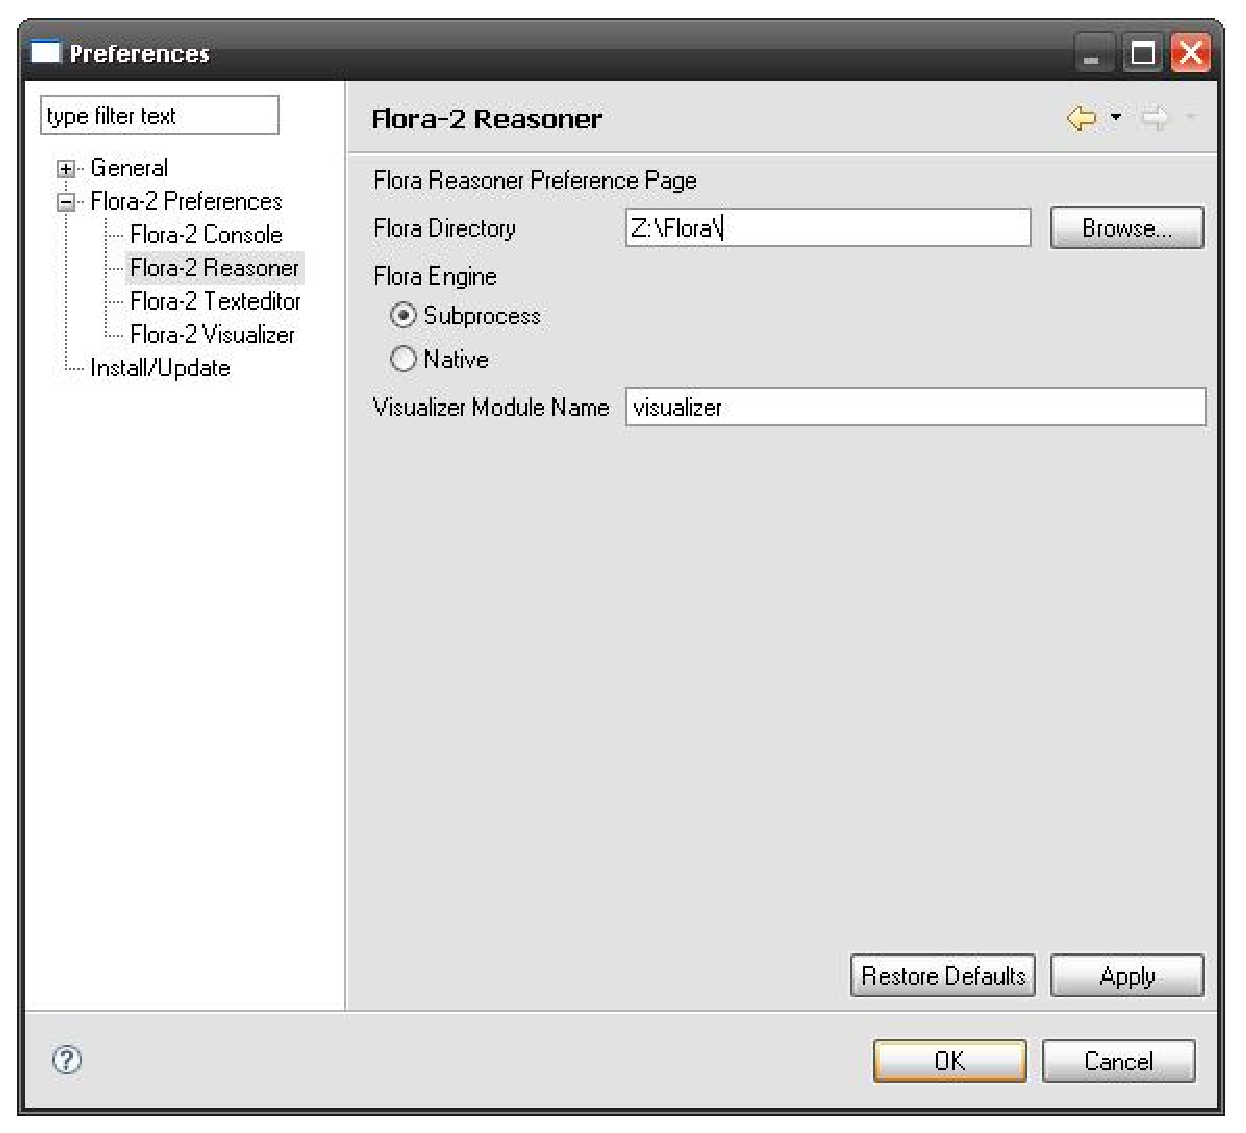
\includegraphics[width=0.75\textwidth]{preferencepage_reasoner}
	\caption{\FLORA Reasoner Preference Page}
	\label{fig:preferencepage_reasoner}
\end{figure}

\begin{itemize}
\item \emph{Flora Directory}  \\
  The directory where \FLORA is located.

\item \emph{Interprolog Engine}  \\
  Interprolog provides two engines: \emph{Native} and \emph{Subprocess}.
  The native engine is faster, but it does not work well under Linux.

\item \emph{Visualizer Module Name}\\
  The name of the \FLORA module through which the reasoner communicates
  with the visualizer. You can leave the default unchanged unless the same
  name is already used in your \FLORA application.
\end{itemize}

After applying the changes the visualizer
is ready for use. The user can talk to the \FLORA reasoner through
\FVIZ Console and also (in a limited way) by directly manipulating the
objects in \FVIZ  Class Diagram View. We describe these components below.

\section{Working with the Visualizer}

\begin{figure}[tbh]
	\centering
		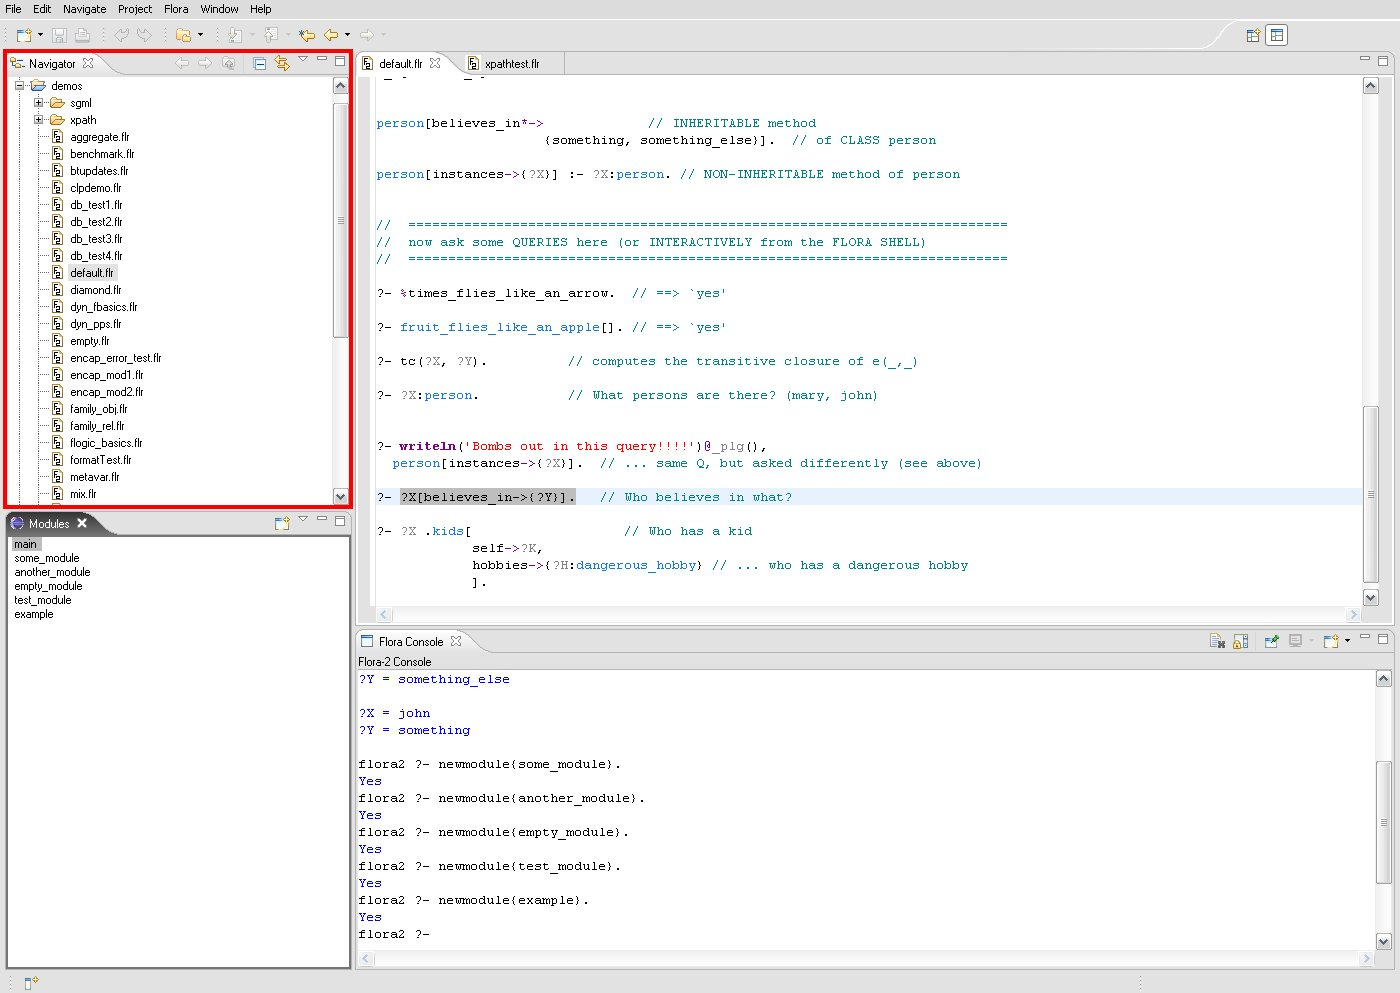
\includegraphics[width=0.95\textwidth]{fviz_navigator}
	\caption{\FVIZ Navigator}
	\label{fig:fviz_navigator}
\end{figure}

To begin working with \FVIZ, Eclipse (or the \FVIZ standalone application)
has to be started. You will be asked to select a directory for a
workspace. This location specifies where the projects and preferences will
be stored.  To create a new project, select
\emph{New} $\rightarrow$ \emph{Project} from the file menu.
A dialog will appear and prompt for
the name of a new project.  For more information have a look at the Eclipse
help\footnote{
  \url{http://help.eclipse.org/help32/index.jsp?topic=/org.eclipse.platform.doc.user/gettingStarted/qs-07a.htm}
}.

For each project, Eclipse creates a subdirectory in the directory of
the workspace; it has the same name as the project. All project's files
will be stored in this directory.

Once the project is created, you can either import existing \FLORA files or
use \FVIZ to create new knowledge bases.
Files can be imported by choosing the
\emph{File} $\rightarrow$ \emph{Import} menu item.
A dialog will appear and lead you through the process of
importing files to the project.
The imported files will then be copied to your project directory.

Note that \FVIZ will work \emph{only} with the copies of the files stored
in the project subdirectory. If these files were created via import and you
modify the source files (from which the import was created)
then these changes will \emph{not} be propagated to
the project.

Also, if you copy a file into a project directory \emph{manually} outside
of Eclipse then this new file will not automatically be made part of the
project.  To include it in the project, you need to use the mouse to
select the requisite
files in the \FVIZ Navigator View and then press \emph{F5}.
For more information on importing, have a look at the Eclipse help\footnote{
  \url{http://help.eclipse.org/help32/topic/org.eclipse.platform.doc.user/gettingStarted/qs-31a.htm}
}.

To create a new file, choose
\emph{New} $\rightarrow$ \emph{Other...}
$\rightarrow$ \emph{File} from the \emph{File} menu. 
Then give the name to the new file (do not forget the file ending
e.g. \emph{new\_file.flr}) and choose a project.\footnote{
\url{http://help.eclipse.org/help32/topic/org.eclipse.platform.doc.user/reference/ref-39.htm}
%%
}
%%
The files can then be edited with the \FVIZ Text Editor.
See Section~\ref{sec:texteditor} to learn more about the editor.

After creating the necessary \FLORA modules, we can start working with the
visualizer. The system allows the user to load, run, and query \FLORA
knowledge bases through \FVIZ Console and to visualize class diagrams
and object definitions. These capabilities are described in the following
sections.

To learn more about the Eclipse workbench see the \emph{Workbench User Guide} at
\url{http://help.eclipse.org}.

\section{The \FVIZ Console}
\label{sec:consoleview}

\begin{figure}[tbh]
	\centering
		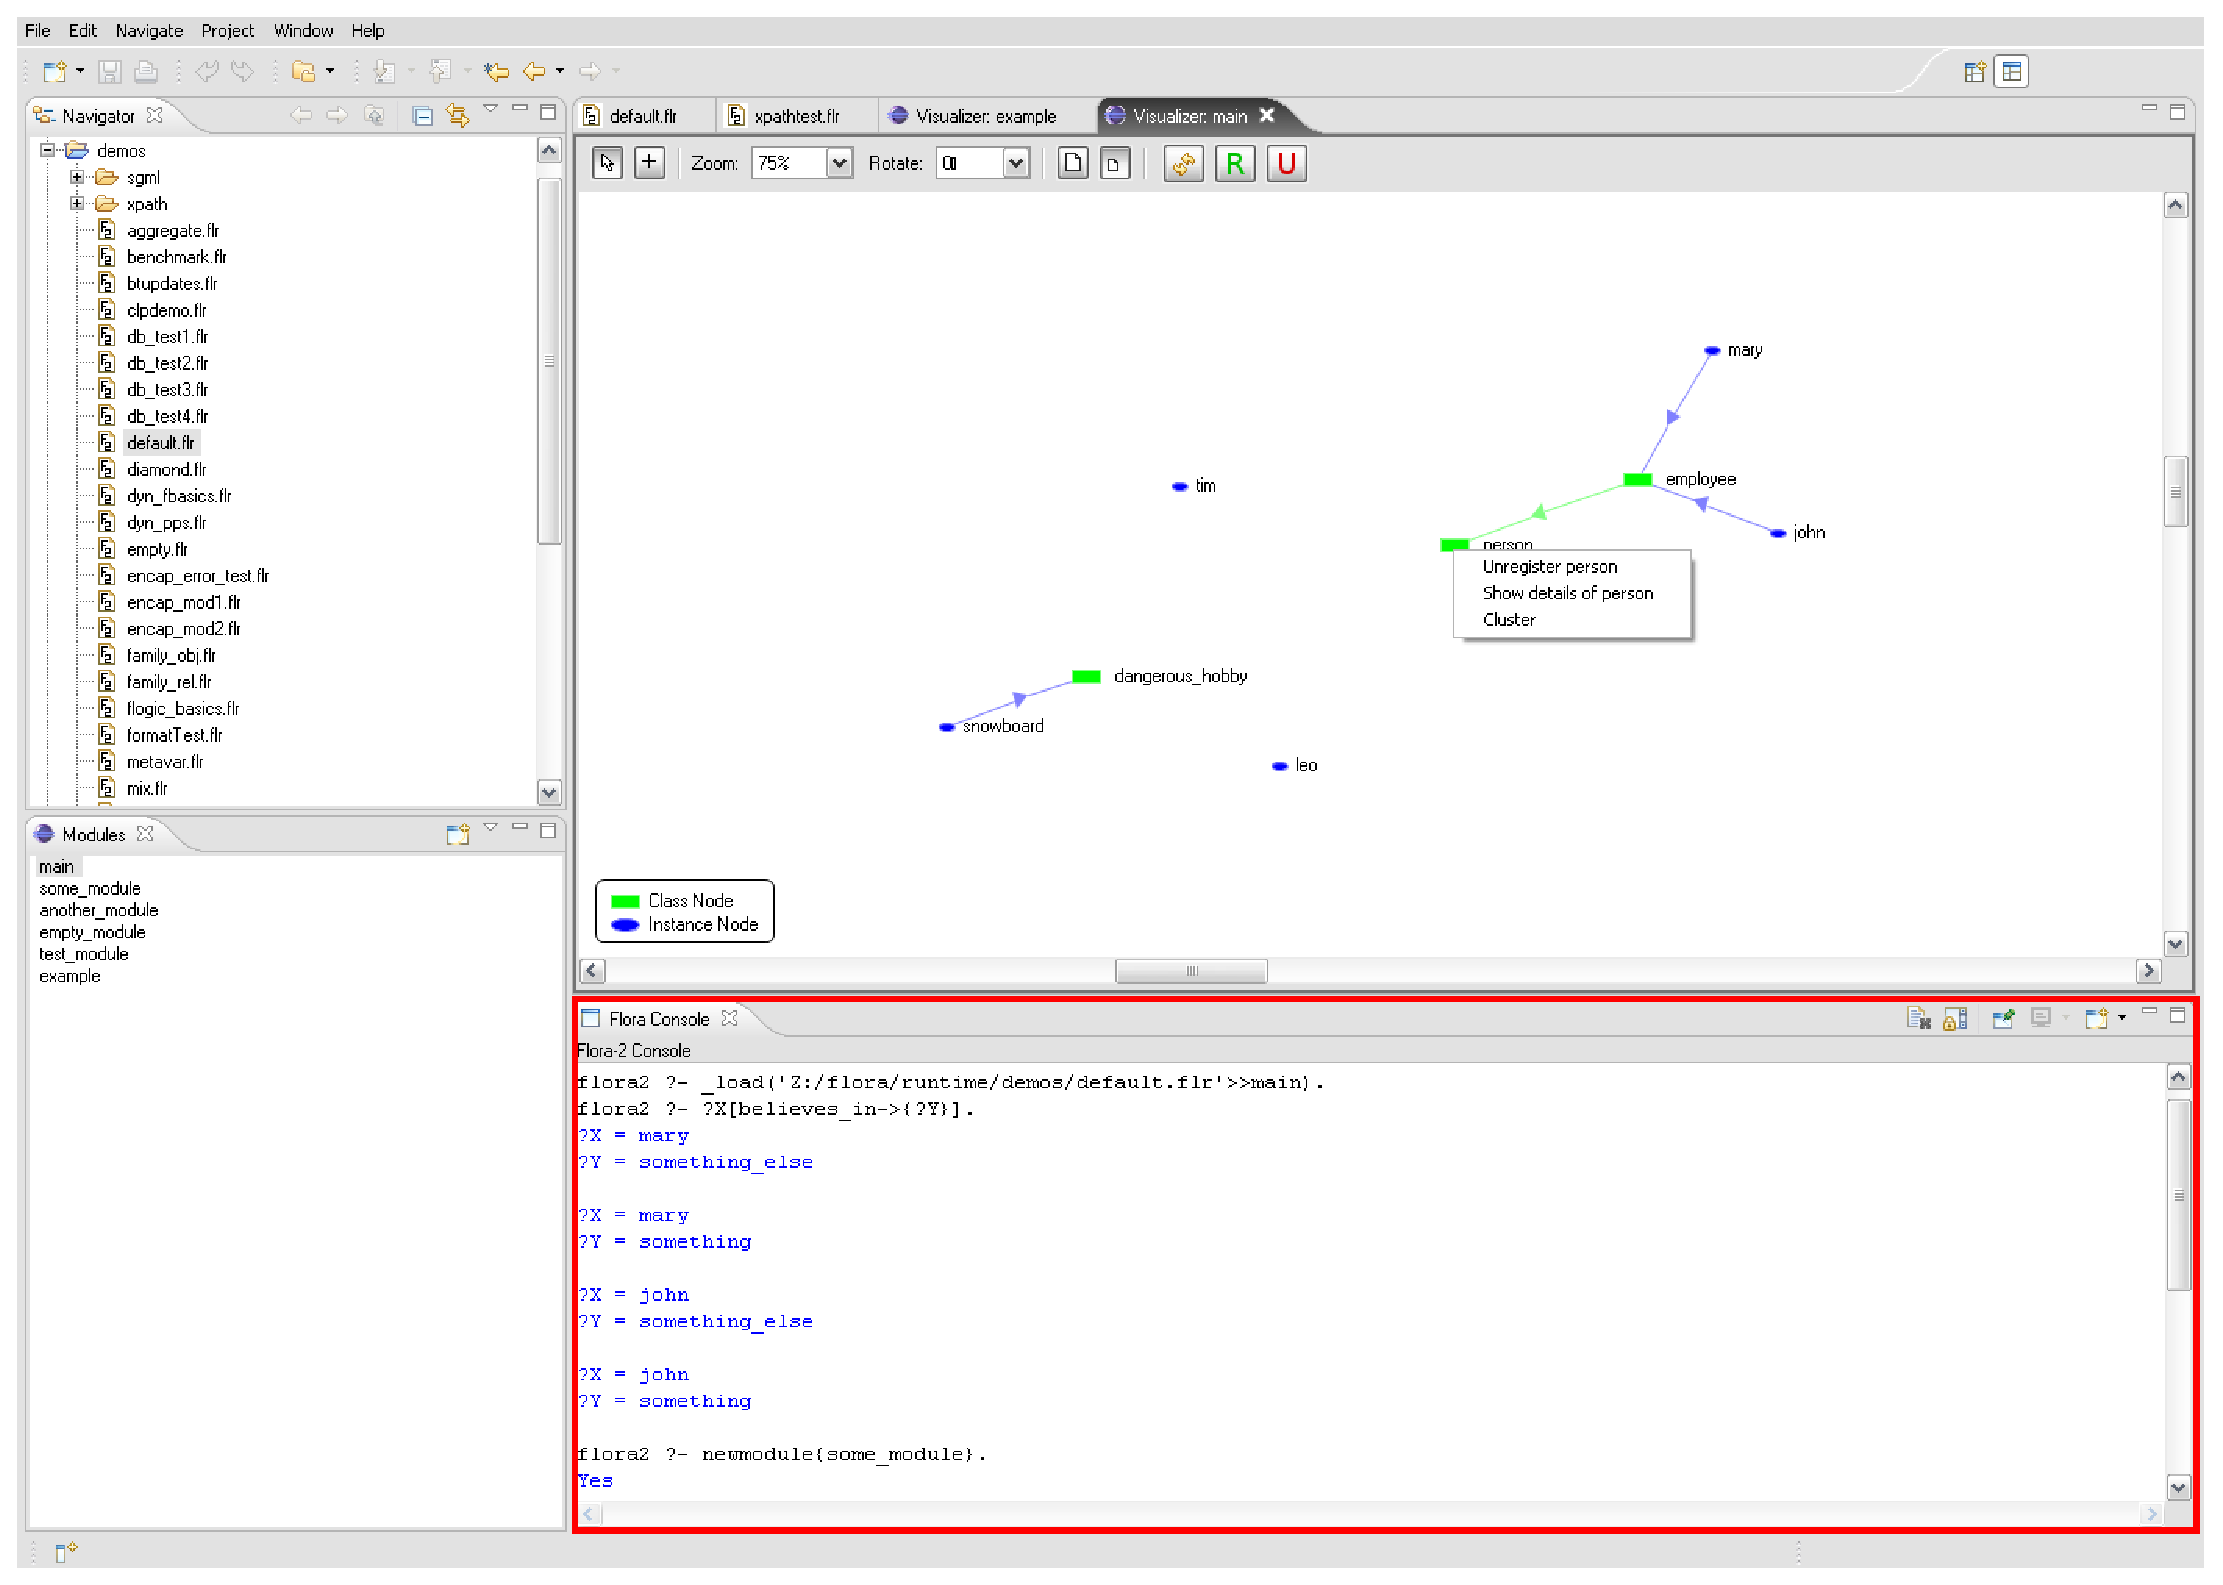
\includegraphics[width=0.95\textwidth]{fviz_console}
	\caption{\FVIZ Console View}
	\label{fig:fviz_console}
\end{figure}

The \FVIZ Console allows you to communicate with the current \FLORA session.
All \FLORA commands and queries are available through the console.

\subsection{Configuration}
\label{sec:consoleview_configuration}

It is not necessary to configure the console unless you dislike the colors
with which the visualizer highlights text. To change the colors, choose
the \FLORA Console Preference page where you can alter the defaults:
\begin{itemize}
\item \emph{Default color}  \\
This is used to highlight user input.
\item \emph{Response color}  \\
  This color is used for normal \FLORA feedback.
\item \emph{Error color} \\
  This color is used for error messages.
\end{itemize}

\subsection{Usage}
\label{sec:consoleview_usage}

The \FVIZ Console 
parses user commands and sends them to the \FVIZ Reasoner.
The console then displays the results, errors, and other possible feedback.
You may also see some commands that you did not type: these are
issued by the visualizer.

\section{The \FVIZ Module View}
\label{sec:moduleview}

\begin{figure}[tbh]
	\centering
		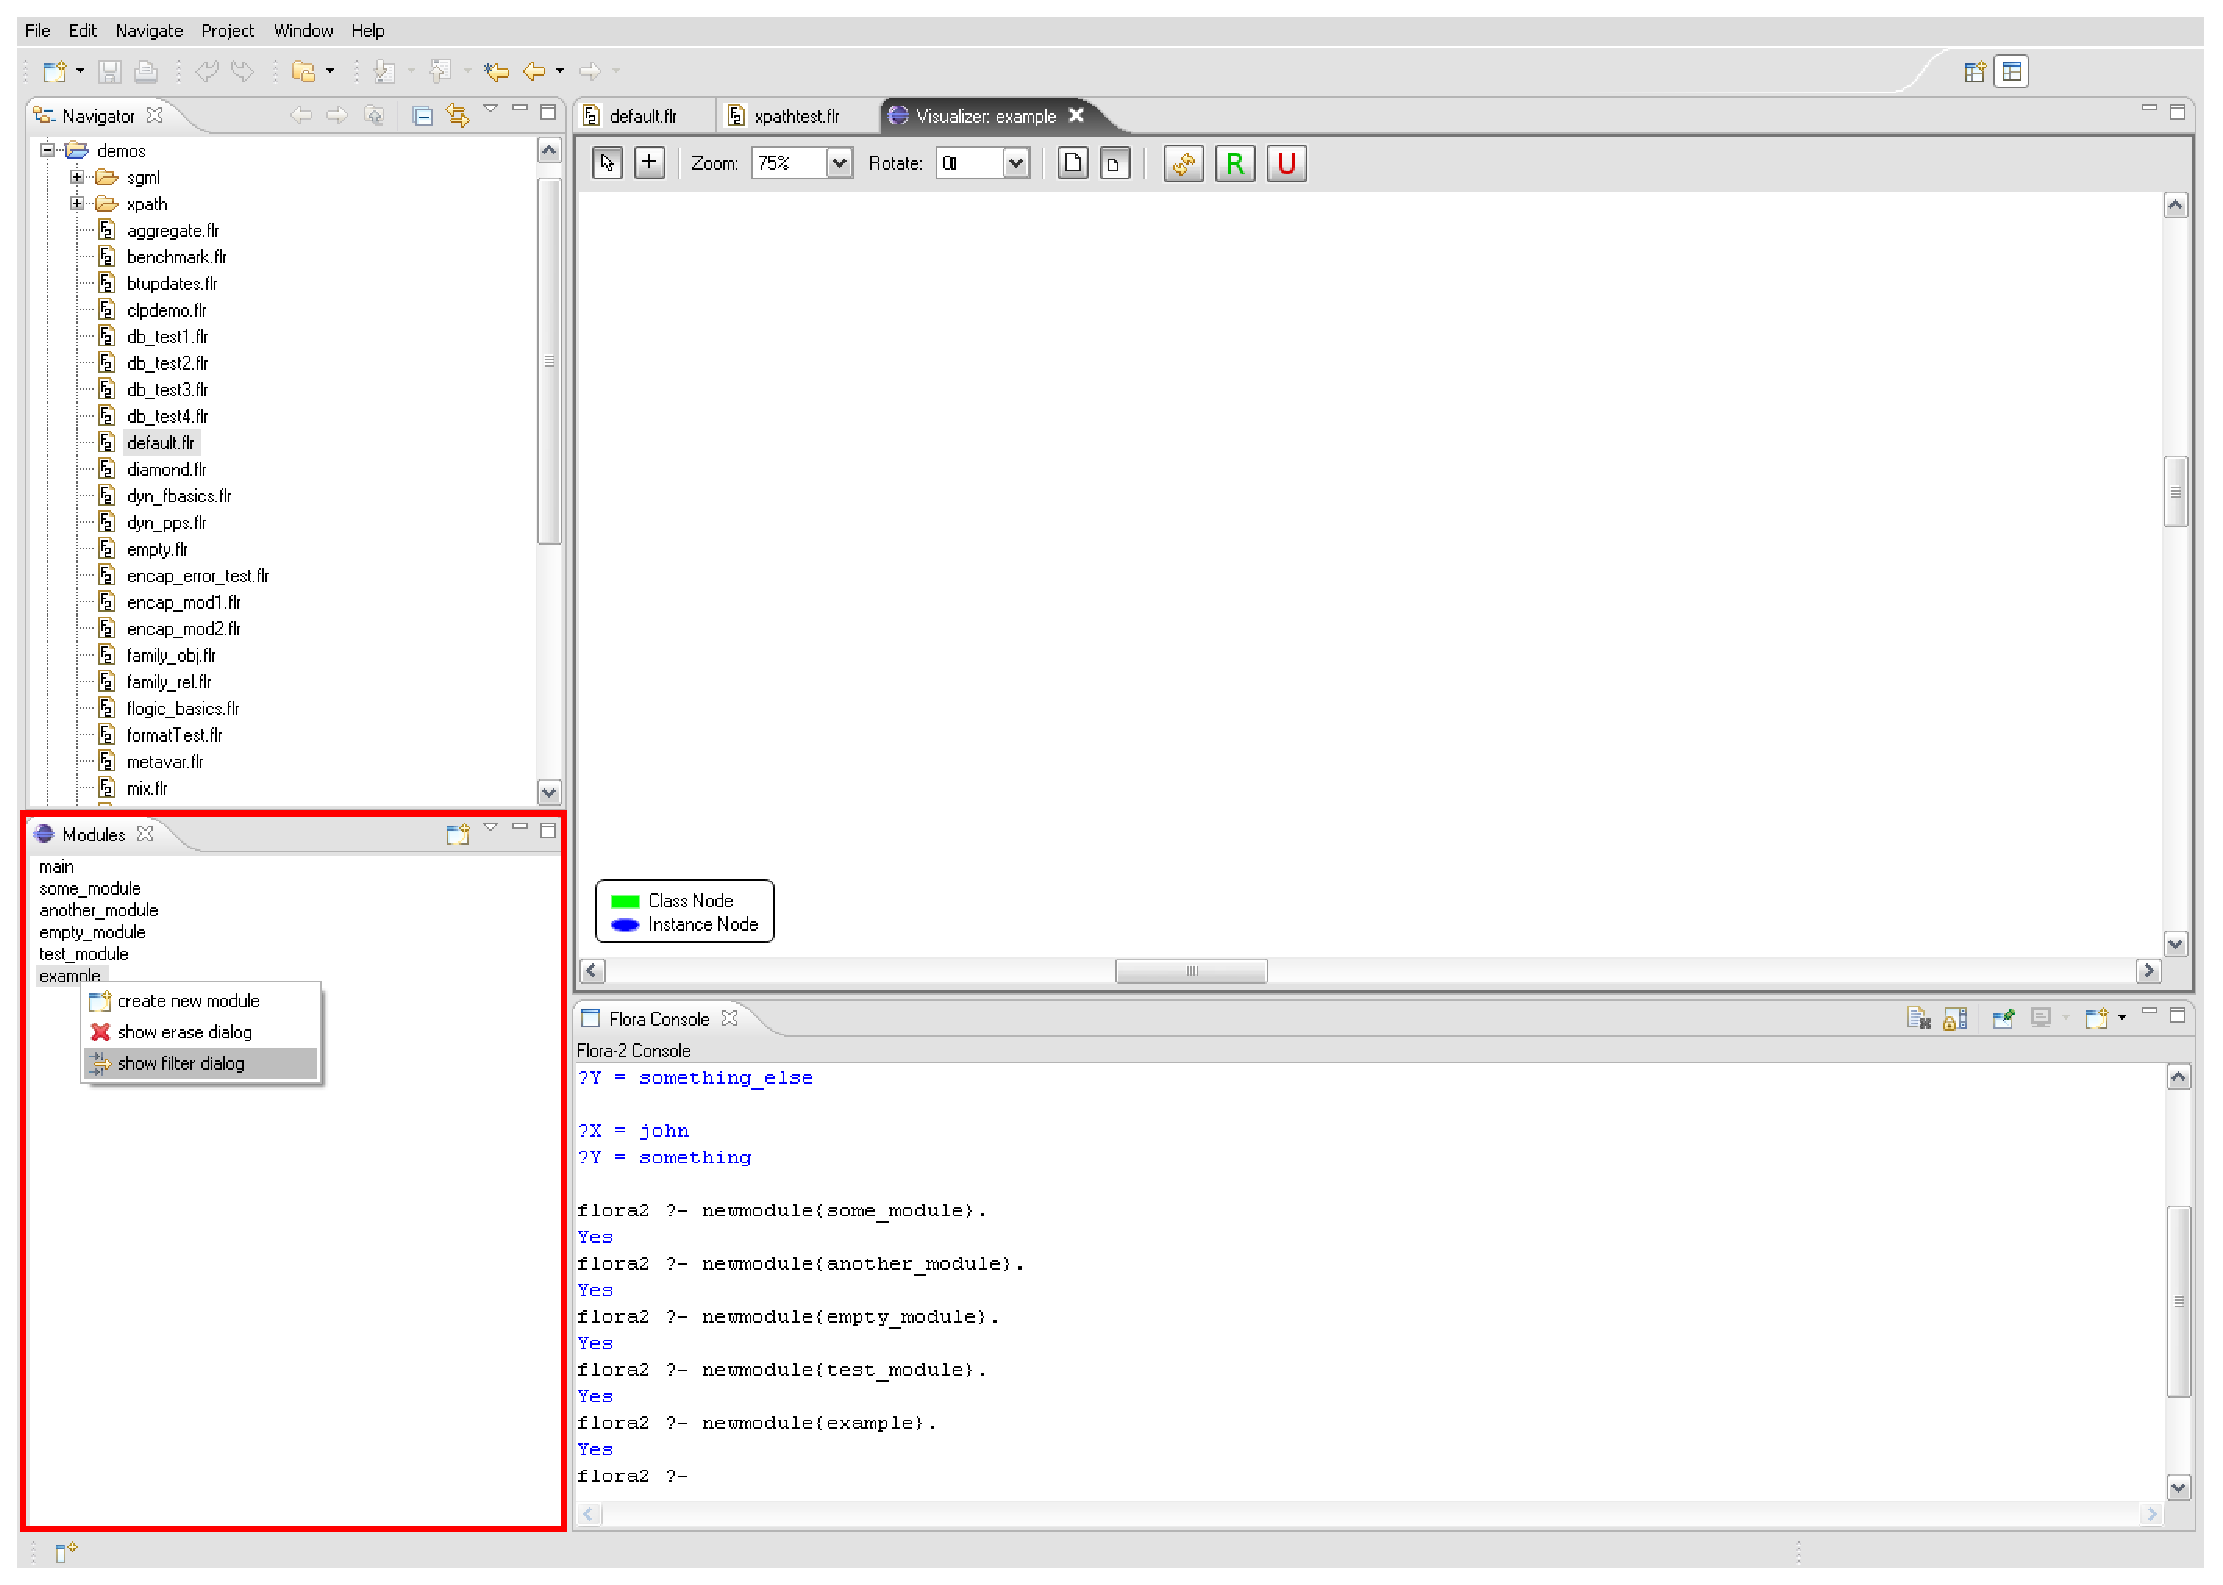
\includegraphics[width=0.95\textwidth]{fviz_module}
	\caption{\FVIZ Module View}
	\label{fig:fviz_module}
\end{figure}

The \FVIZ Module View shows all currently loaded \FLORA modules (except the
module which is used for the visualizer itself).
This view does not have configuration options.

\subsection{Usage}
\label{sec:moduleview_usage}

The module view supports
creation, deletion, and hiding of \FLORA modules. It also supports
drag-and-drop idioms for loading and adding \FLORA knowledge to modules.

\subsubsection{Loading and Adding Files}
\label{sec:moduleview_usage_loadingandadding}

\FLORA files imported into a visualizer project appear in the Navigator
View of the \FVIZ. Any such file can be dragged with the mouse into any of the
modules shown in the Module View. When you drop such a file into a module,
a context menu pops up and you can select one of the following operations:

\begin{itemize}
\item \emph{load to module and erase registered objects}\\
  This option erases all registered object and loads the file to the
  specified module. The current contents of the module is erased as well.
  This corresponds to the {\tt \_load} command in \FLORA.

  The registered objects mentioned here are the objects and classes that
  are supposed to be displayed in the \FVIZ Class Diagram View. See
  Section~\ref{sec:visualizerview_usage_registration} for more details on
  the concept of registered objects.

\item \emph{load to module and keep registered objects}\\
  This option loads the file into the specified module and erases the
  module's earlier contents, but it preserves the registered objects.
  This operation is useful when you change a \FLORA file and want to reload
  it into the same module where it was before. In that case, the class
  diagram for that module will be updated.

\item \emph{add to module and keep registered objects}\\
  This action corresponds to the {\tt \_add} command of \FLORA. It adds
  knowledge to an existing module without erasing the old contents. 
  The registered objects are preserved and the class diagram is updated.
\end{itemize}

\subsubsection{Creating New \FLORA Modules}
\label{sec:moduleview_usage_createmodules}

To create a new \FLORA module using the \FVIZ Module View,
click the \emph{create new module} button or use the context menu, which
pops up when you 
right-click on the list of modules.
This causes a display of a dialog where you can specify  the name of a
module to be created.
Click \emph{OK} to confirm the request.
This is equivalent to the {\tt newmodule} command. 

\subsubsection{Erasing \FLORA Modules}
\label{sec:moduleview_usage_erasemodules}

To erase an existing module using the Module View, choose
\emph{show erase dialog} from the context menu, which pops up when you
right-click over the module list. In the dialog that is then displayed, you
can check the modules to be erased and then click the OK emm button.
This is equivalent to the {\tt erasemodule} command. 


\subsubsection{Hiding  \FLORA modules}
\label{sec:moduleview_usage_filtermodules}

To hide selected \FLORA modules from the \FVIZ Module View, use
the \emph{show filter dialog} in the context menu.
he dialog box that is then displayed allows the user to check the modules
to be hidden. Note that this does not erase those modules---just hides them
from the view.

\section{The \FVIZ Text Editor}
\label{sec:texteditor}

\begin{figure}[tbh]
	\centering
		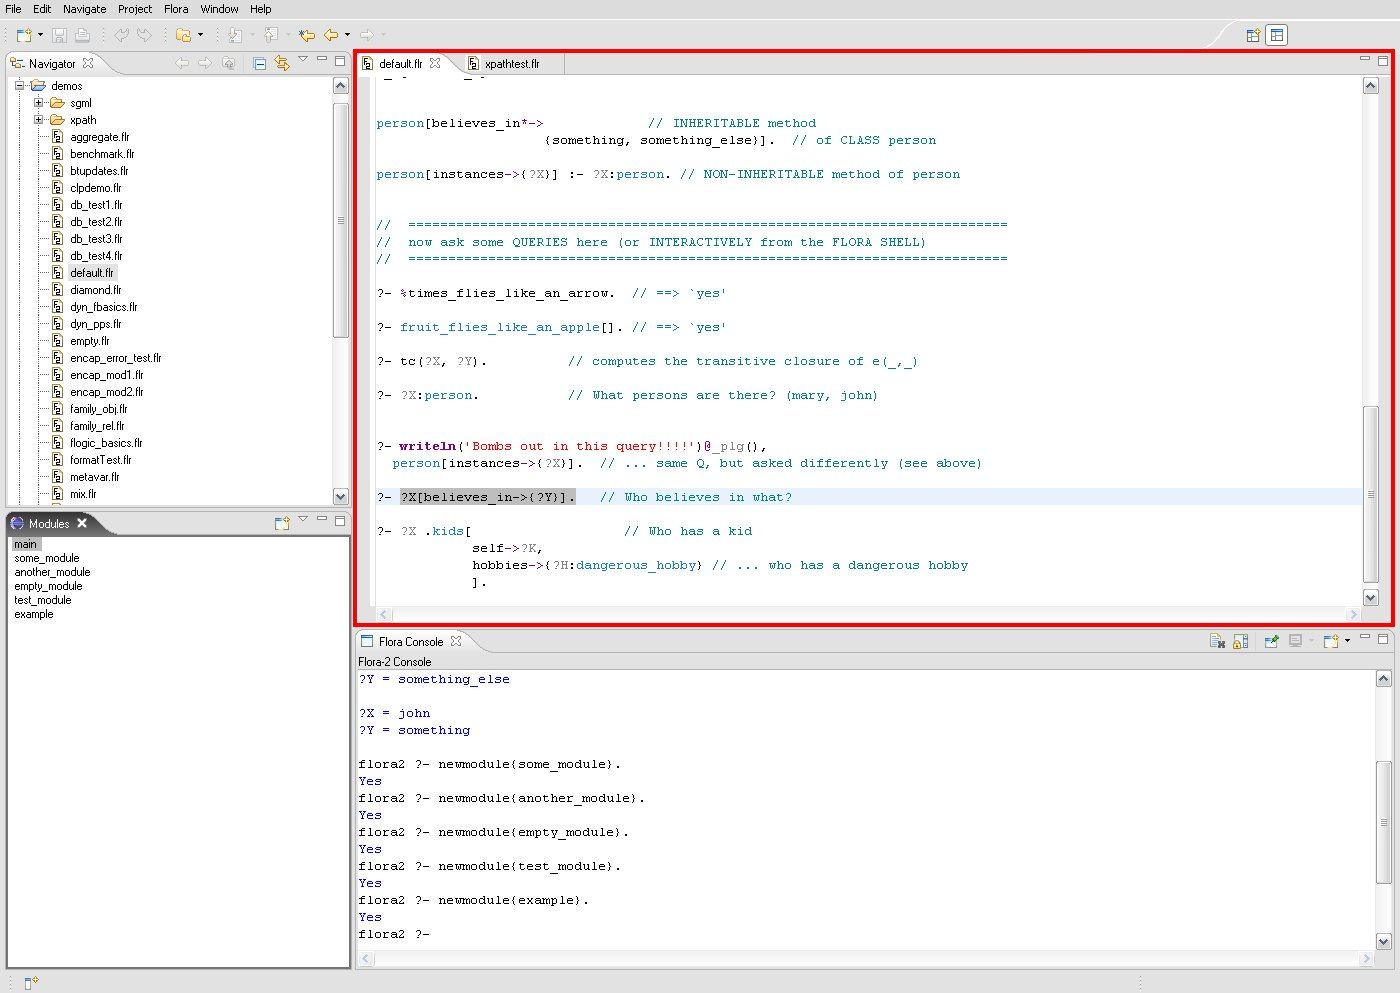
\includegraphics[width=0.95\textwidth]{fviz_editor}
	\caption{\FVIZ Text Editor}
	\label{fig:fviz_editor}
\end{figure}

The \FVIZ Text Editor is used to edit \emph{.flr} files. It supports
syntax-highlighting, auto-indentation, and text-formatting.

\subsection{Configuration}
\label{sec:texteditor_configuration}

There is no need to configure the text editor unless you dislike its
default settings. If you decide to change those settings,
the \FVIZ Text Editor configuration page is located at the \emph{Flora-2
  Preferences} $\rightarrow$ \emph{Flora-2 Text Editor} menu item.
The preference page allows the user to change the following settings:
\begin{itemize}
\item \emph{Tab width} \\
  The number of space characters which are displayed in place of a tab
  character.

\item  \emph{Tab type} \\
  If set to \emph{Tab}, the \FVIZ Text Editor displays \lstinline|'\t'| in
  place of a tab.  If set to \emph{Space}, the tab is displayed as a
  sequence of spaces. The number of the spaces is controlled by the aforesaid
  tab width parameter.


\item \emph{Colors}\\
  This options allow to change the colors of different text tokens:
  strings, numbers, keywords, etc.
\end{itemize}

\subsection{Usage}
\label{sec:texteditor_usage}

The \FVIZ Text Editor is specifically designed for the \FLORA
syntax. It automatically highlights the various syntactic components
and it indents text items to their proper position when the user hits the
\emph{Return} key.
Also, when the user hits the \emph{TAB} key then the line marked by the
cursor is also indented in accordance with the \FLORA syntactic conventions.

\subsection{Menu}
\label{sec:texteditor_menu}

When \FVIZ text editor is active,
\FLORA menu is extended with the following actions:

\begin{itemize}
\item \emph{Format}\\
  This action formats the highlighted (or the whole if nothing is
  highlighted) text.  This corrects the indentations and beautifies the
  spaces between tokens.

\item \emph{Open Buffer}\\
  This action opens a new blank buffer in the editor and allows the user to
  start typing new text. This text can be saved as usual, through the
  \emph{File} $\rightarrow$ \emph{Save as} menu item.

\item \emph{Add Region to Module}\\
  This action adds the rules and the facts in the
  selected text region of the currently active
  \FVIZ Text Editor to a \FLORA module.
  To specify the module, a dialog pops up.

\item \emph{Add Region}  \\
  This action adds the rules/facts of
  the selected text region of the current \FVIZ Text
  Editor to \FLORA's module {\tt main}.

\item \emph{Load Region to Module} \\
  This action loads the rules and facts in the
  selected text region of the currently active
  \FVIZ Text Editor to a
  \FLORA module.  A dialog pops up where the user can specify the desired
  module.

\item \emph{Load Region}  \\
  This action adds the contents of
  the selected text region of the currently active Text Editor to
  the \FLORA module {\tt main}. 

\item \emph{Execute Region as a Query}  \\
  This action executes the selected text of the current \FVIZ Text Editor
  as a query.

\end{itemize}

\section{The \FVIZ Class Diagram View}
\label{sec:visualizerview}

\begin{figure}[tbh]
	\centering
		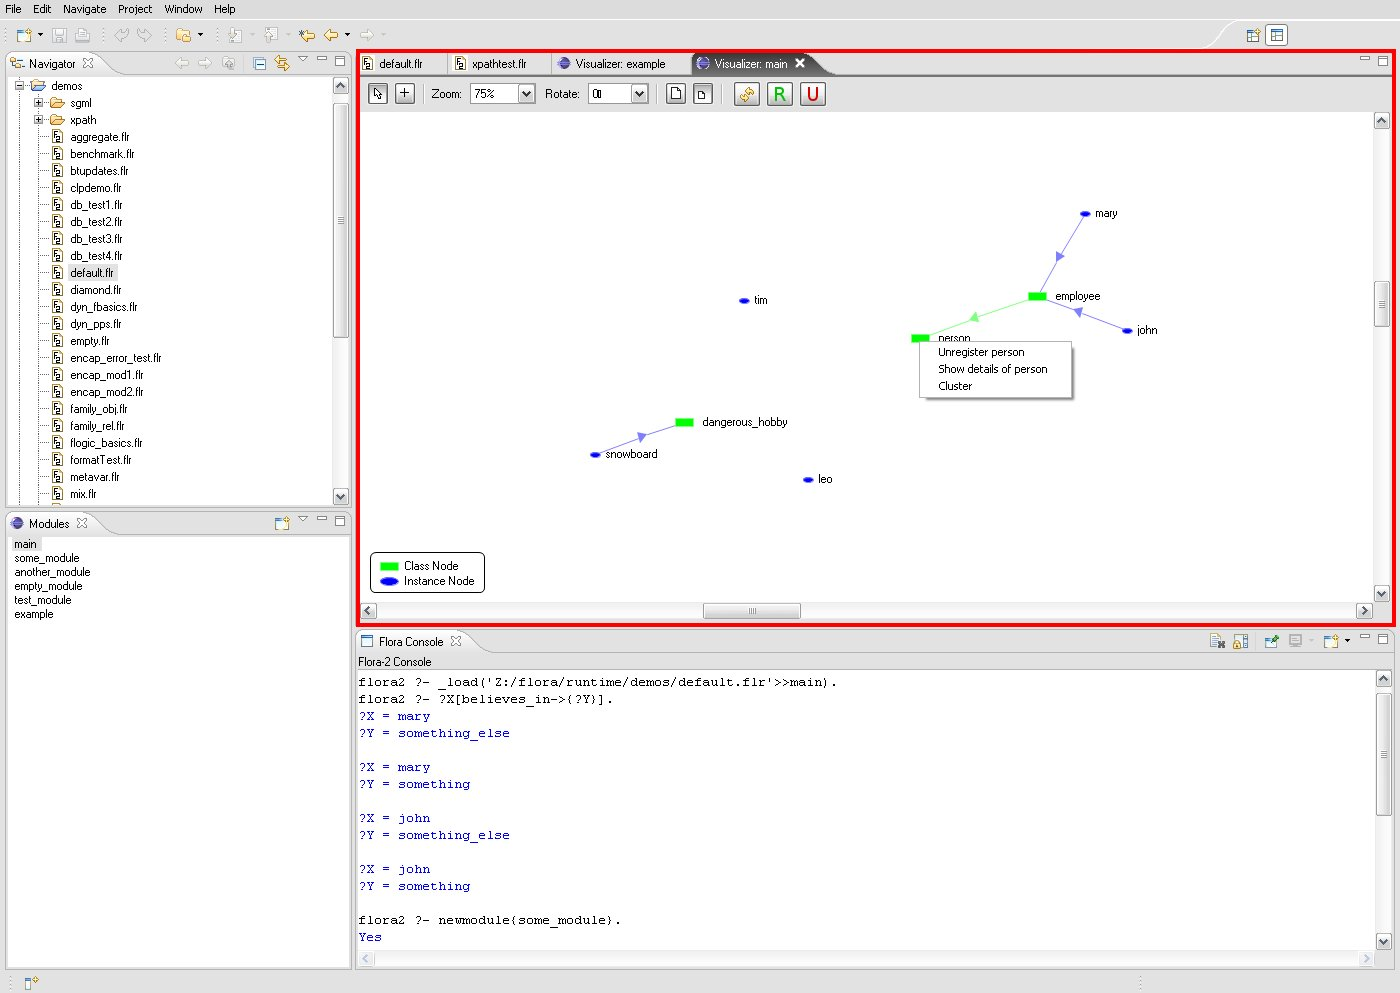
\includegraphics[width=0.95\textwidth]{fviz_viz}
	\caption{\FVIZ Class Diagram View}
	\label{fig:fviz_viz}
\end{figure}

The \FVIZ Class Diagram View shows the class hierarchy of the selected
\FLORA module. Only the registered objects are displayed. The concept of
registered objects is explained in
Section~\ref{sec:visualizerview_usage_registration}.

\subsection{Configuration}
\label{sec:visualizerview_configuration}

The class diagram view does not need to be configured. But the following
parameters can still be changed though the page accessible by selecting
\emph{Flora-2 Preferences}
$\rightarrow$ \emph{Flora-2 Visualizer}.
\begin{itemize}
\item \emph{Class/instance Node Colors} 

\item \emph{Zoom level}  \\
  This allows the user to zoom the class diagram in and out.

\item \emph{Node Size}  \\
  The size of the nodes that represent classes and instances. 

\item \emph{Use Instance Cluster}  \\
  If checked the graph makes use of instance clusters. This means that the
  graph will contain one big blob to represent all instances of each class,
  if the number of instances exceeds the cluster size (see next).
  This is useful when the graph can have too many instances.

\item \emph{Minimum Cluster Size}  \\
  The number of instances in a class
  at which the graph shows an instance cluster instead of
  individual instances for the class.
  The \FVIZ Class Diagram View allows one to
  dynamically switch between clustered and unclustered views.
\end{itemize}

\subsection{Usage}
\label{sec:visualizerview_usage}

Each \FVIZ Class Diagram View shows a class hierarchy (restricted to
registered objects) for
a particular \FLORA module. A \FVIZ Class Diagram View for a module
can be opened by
clicking on the module in the \FVIZ Module View (see
Section~\ref{sec:moduleview}).

\subsubsection{Registering Objects for Display in Class Diagram Views}
\label{sec:visualizerview_usage_registration}

\index{registration}
In general, a \FLORA knowledge base can have an infinite number of objects
and classes. Clearly, no graphical display can show this kind of hierarchies.
However, in most cases users want to focus only on a small subset of the
hierarchy.  \FVIZ lets users specify this focus through the mechanism of
\emph{registration}.

There are two ways to register objects for display. The simplest one is to
use the Class Diagram View, which provides the \emph{R} and \emph{U}
buttons for registering and deregistering objects. This interface is quite
effective for quick experiments, but it is too weak and inflexible, since
it requires that the user provide the list of objects to be registered.

A more flexible and permanent mechanism is to use the {\tt \%register} and
{\tt \%unregister} methods of the visualizer module.  For instance, to
register objects \emph{a}, \emph{b}, and \emph{c}, in a \FLORA
module {\tt foobar} one could put the following query in a \FLORA program
(or to execute it at command prompt):
%% 
\begin{verbatim}
  ?- foobar[%register([a,b,c])]@visualizer.
\end{verbatim}
%% 
Here we assume that \FVIZ uses the module called {\tt visualizer}  
to communicate with \FLORA. This module is specified when you configure
\FVIZ, as described in Section~\ref{sec:reasoner}.
If this is specified then the user will not need to register the
corresponding objects by clicking the \emph{R} button each time the
visualizer starts.

There is an even more powerful way of specifying which objects to register.
To this end, the user can define a \emph{unary} predicate, say {\tt
  myregobjs}, and define it via the usual \FLORA deductive rules.  It is
user's responsibility, however, to ensure that the number of objects thus
specified is finite (otherwise, the visualizer will hang).
Then the user can include the following query in the source file:
%% 
\begin{verbatim}
  ?- foobar[%register(${myregobjs(?)})]@visualizer.
\end{verbatim}
%% 
This query will register every object that is returned as an answer to the query
%% 
\begin{verbatim}
 ?- myregobjs(?X).
\end{verbatim}
%% 

\index{unregistration}
\index{deregistration}
The method {\tt \%unregister} can be used to remove objects from the Class
Diagram View.  It also can take a list of objects or a unary predicate.

\subsubsection{Context Menu}
\label{sec:visualizerview_usage_contextmenu}

The nodes in the Class Diagram View display context menus when one
right-clicks on them. The context menu contains the following items:
%%
\begin{itemize}
\item \emph{Unregister}\\
  This action deregisters the object under the context menu.

\item \emph{Show details} \\
  This action opens a \emph{Details Dialog} with two panes showing the
  values and types of the attributes of the object under the menu. For
  nodes that represent instance-clusters, right-clicking opens a dialog
  listing all instances in the cluster. You can double-click on an instance
  to open the \emph{Details Dialog} for that object.  The \emph{Details
    Dialog} also pops up when one double-clicks on an node that represents
  an object.

\item \emph{Cluster}\\
  This action applies only to \FLORA class nodes. It redraws the graph and
  clusters the instances of that class.

\item \emph{Uncluster}\\
  This action applies only to \FLORA class nodes and to cluster nodes. It
  redraws the graph and shows individual instances of the class instead of
  a single cluster node.
\end{itemize}

It should be noted that some commands executed from the console may affect
the class diagram but \FVIZ might not be able to detect this.
For this purpose, the Class Diagram View provides a \emph{Redraw} button. 


\paragraph{ACKNOWLEDGEMENTS.}

We would like to thank Mick Kerrigan for developing JPowerGraph and for
helping along with this project.




%%%%%%%%%%%%%%%%%%%%%%%%%%%%%%%%%%%%%%%%%%%%%%%%%%%%%%%%%%%%%
%% BIBLIOGRAPHY AND OTHER LISTS
%%%%%%%%%%%%%%%%%%%%%%%%%%%%%%%%%%%%%%%%%%%%%%%%%%%%%%%%%%%%%
%% A small distance to the other stuff in the table of contents (toc)
\addtocontents{toc}{\protect\vspace*{\baselineskip}}

%% The Bibliography
%% ==> You need a file 'literature.bib' for this.
%% ==> You need to run BibTeX for this (Project | Properties... | Uses BibTeX)
%%\clearpage
\addcontentsline{toc}{section}{Bibliography} %'Bibliography' into toc
\nocite{*} %Even non-cited BibTeX-Entries will be shown.
\bibliographystyle{alpha} %Style of Bibliography: plain / apalike / amsalpha / ...
\bibliography{literature} %You need a file 'literature.bib' for this.

%% The List of Figures
\clearpage
%%\addcontentsline{toc}{section}{List of Figures}
%%\listoffigures

%% The List of Tables
%\clearpage
%\addcontentsline{toc}{section}{List of Tables}
%\listoftables


%%%%%%%%%%%%%%%%%%%%%%%%%%%%%%%%%%%%%%%%%%%%%%%%%%%%%%%%%%%%%
%% APPENDICES
%%%%%%%%%%%%%%%%%%%%%%%%%%%%%%%%%%%%%%%%%%%%%%%%%%%%%%%%%%%%%
%\appendix
%% ==> Write your text here or include other files.

%\input{FileName} %You need a file 'FileName.tex' for this.

\end{document}
